\label{chap:results}

This chapter presents the quantitative and qualitative evaluation of the proposed fastener detection and counting framework. The evaluation is structured into two primary phases: (1) controlled benchmarking on the physical mock-up environment, and (2) a real-world Proof of Concept (PoC) demonstration on a simplified conveyor system. \\

During the model development and quantitative benchmarking phase, the full-scale industrial conveyor belt infrastructure was still under concurrent development by the mechanical and electrical engineering teams. Consequently, raw performance metrics were captured using the controlled physical mock-up environment described in Chapter~\ref{sec:dataset}. Despite this constraint, the final system was validated through a PoC deployment on a simple conveyor setup that closely mimics the target operational environment. This progression demonstrates the model's ability to generalize from mock-up and public training data to near-actual deployment conditions.

\section{Quantitative Benchmarking on Mock-up Environment}
To evaluate the speed--accuracy trade-off of the proposed architecture, we conducted rigorous benchmarking across two distinct scenarios representing varying levels of industrial complexity: a \textbf{Medium Case} ($\approx$\,85 fasteners) and a \textbf{Hard Case} ($\approx$\,430 fasteners). All models were evaluated under identical conditions to ensure a fair comparison.

\subsection{Medium Case Performance ($\approx$\,85 Fasteners)}
The medium case represents a standard operational load with moderate object density and minimal occlusion. As shown in Table~\ref{tab:benchmark_medium}, the proposed \textbf{YOLO11-GED} model achieves the highest throughput (100.8\,FPS) and the lowest latency (10.4\,ms) while maintaining perfect counting accuracy (85/85).

\begin{table}[htbp]
    \centering
    \caption{Benchmarking Summary: Medium Case ($\approx$\,85 Fasteners)}
    \label{tab:benchmark_medium}
    \begin{tabular}{lccccc}
        \toprule
        \textbf{Model Name} & \textbf{Avg FPS} & \textbf{Avg Latency} & \textbf{GPU Util} & \textbf{CPU Util} & \textbf{Counted} \\
        \midrule
        \textbf{YOLO11-GED (Proposed)} & \textbf{100.8} & \textbf{10.4 ms} & \textbf{40.4\%} & \textbf{7.9\%} & \textbf{85} \\
        YOLO11-s             & 93.8           & 10.9 ms            & 37.5\%          & 8.4\%           & 84             \\
        YOLO11-m             & 106.7          & 9.6 ms             & 39.2\%          & 7.9\%           & 78             \\
        RT-DETR              & 31.7           & 31.7 ms            & 54.6\%          & 8.2\%           & 82             \\
        YOLO26m              & 99.6           & 10.2 ms            & 42.2\%          & 8.6\%           & 84             \\
        \bottomrule
    \end{tabular}
\end{table}

While YOLO11-m achieves a marginally higher FPS (106.7), it suffers from a significant drop in counting accuracy (78 counted), indicating missed detections likely due to its standard neck architecture struggling with subtle feature distinctions. RT-DETR, while robust, incurs a prohibitive latency penalty (31.7\,ms), rendering it unsuitable for high-speed edge deployment.

\subsection{Hard Case Performance ($\approx$\,430 Fasteners)}
The hard case simulates a high-density, high-throughput industrial scenario with significant object overlapping and occlusion. The results, summarized in Table~\ref{tab:benchmark_hard}, highlight both the resilience of the proposed architecture and the impact of physical setup constraints.

\begin{table}[htbp]
    \centering
    \caption{Benchmarking Summary: Hard Case ($\approx$\,430 Fasteners)}
    \label{tab:benchmark_hard}
    \begin{tabular}{lccccc}
        \toprule
        \textbf{Model Name} & \textbf{Avg FPS} & \textbf{Avg Latency} & \textbf{GPU Util} & \textbf{CPU Util} & \textbf{Counted} \\
        \midrule
        \textbf{YOLO11-GED (Proposed)} & \textbf{89.9}  & \textbf{11.5 ms} & \textbf{37.1\%} & \textbf{8.1\%}  & \textbf{412} \\
        YOLO11-s             & 84.0           & 12.1 ms          & 35.2\%          & 8.5\%           & 421          \\
        YOLO11-m             & 97.0           & 10.5 ms          & 37.9\%          & 8.4\%           & 422          \\
        RT-DETR              & 31.1           & 32.4 ms          & 54.1\%          & 9.3\%           & 377          \\
        YOLO26m              & 90.7           & 11.2 ms          & 40.5\%          & 10.7\%          & 410          \\
        \bottomrule
    \end{tabular}
\end{table}

In this dense scenario, the proposed YOLO11-GED achieved a highly competitive count of 412 fasteners. The slight undercount relative to the ground truth ($\approx$\,430) is primarily attributable to the physical limitations of the mock-up environment rather than algorithmic degradation. Specifically, the camera was positioned relatively close to the conveyor belt, which artificially increased the visual density of the fasteners and reduced their individual pixel footprint. Furthermore, minor camera instability during data capture introduced motion blur, complicating the extraction of fine-grained metallic textures. \\

Despite these suboptimal environmental factors, YOLO11-GED demonstrated remarkable robustness, sustaining an exceptional 89.9\,FPS. In stark contrast, RT-DETR's counting accuracy degraded significantly to 377. This indicates that its transformer-based self-attention mechanisms are highly sensitive to the noise and motion blur introduced by the unstable camera setup. For YOLO11-GED, the integration of the \texttt{EMAc2f} module successfully mitigated occlusion-related false negatives, while \texttt{DySample} preserved the high-frequency edges necessary to distinguish tightly packed fasteners. These domain-specific optimizations effectively compensated for the lack of camera stability, maintaining high counting accuracy without incurring the computational overhead of heavier variants.

\section{Real-World Proof of Concept (PoC) Demonstration}
\label{sec:poc_demo}

While mock-up benchmarking provides controlled, reproducible metrics, the ultimate validation of an industrial vision system lies in its generalization to near-actual operating conditions. To bridge the gap between mock-up testing and final field deployment, a Proof of Concept (PoC) demonstration was conducted on a simplified, functional conveyor belt system that closely replicates the target mechanical and lighting environment.

\subsection{Generalization from Training to Deployment}
A critical challenge in industrial AI is the domain gap between training data and real-world deployment. In this project, the model was trained exclusively on the physical mock-up and public datasets (as the final industrial conveyor was not yet available). Remarkably, the YOLO11-GED model demonstrated strong zero-shot generalization capabilities when deployed on the simple conveyor.

The system successfully:
\begin{itemize}
    \item Recognized diverse fastener types (screws, nuts, bolts) under dynamic, real-world motion blur.
    \item Maintained robust tracking via the ByteTrack integration, preventing double-counting during transient occlusions caused by fastener tumbling.
    \item Executed accurate geometric counting as objects crossed the designated virtual tally line.
\end{itemize}

\subsection{PoC Visual Evidence}
The following figures capture key moments from the PoC demonstration, illustrating the system's real-time detection, tracking, and counting capabilities in a near-actual environment.

\begin{figure}[htbp]
    \centering
    % \fbox{\includegraphics[width=0.9\linewidth]{figures/chapter4/poc_wide.png}}
    \caption{PoC Demonstration: Real-time detection and tracking of fasteners on the simplified conveyor belt. Bounding boxes and unique Track IDs are rendered in real-time.}
    \label{fig:poc_wide}
\end{figure}

\begin{figure}[htbp]
    \centering
    \begin{subfigure}{0.48\textwidth}
        \centering
        \fbox{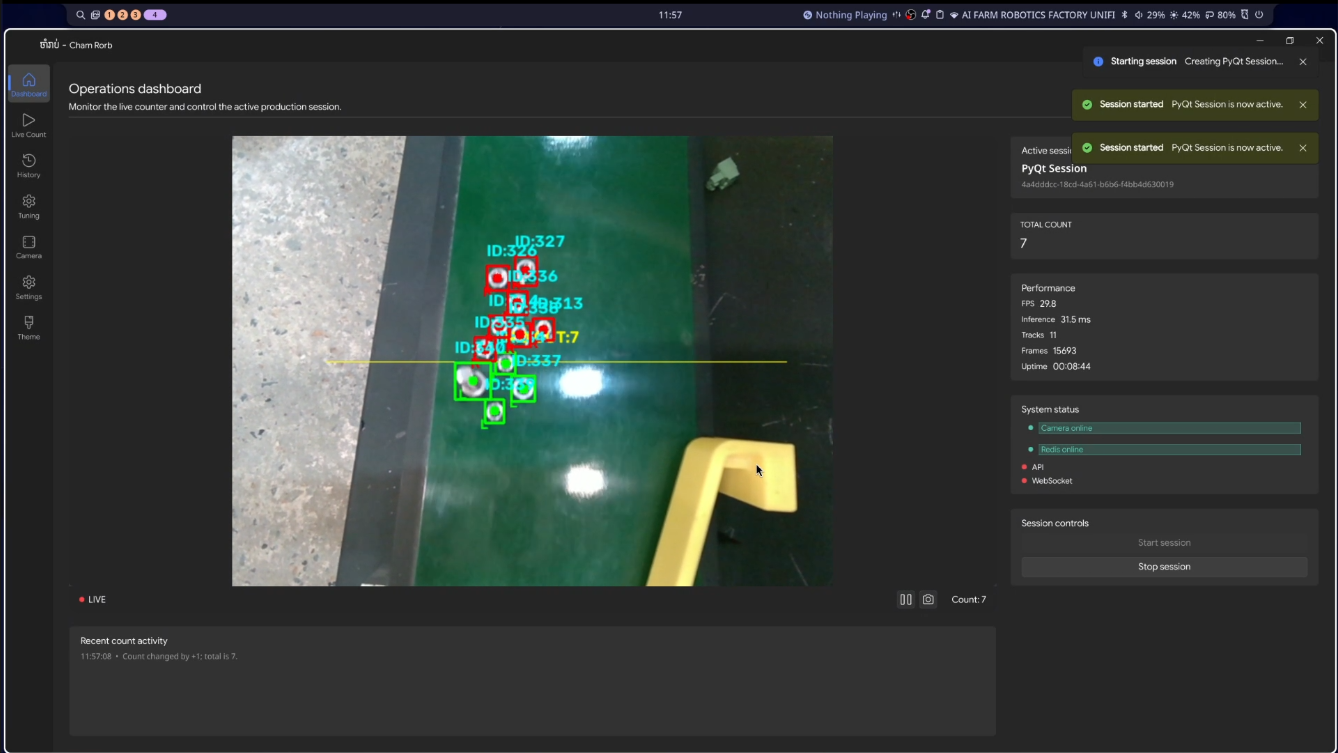
\includegraphics[width=\linewidth]{figures/chapter4/overlapping.png}}
        \caption{High-density fastener grouping}
    \end{subfigure}
    \hfill
    \begin{subfigure}{0.48\textwidth}
        \centering
        \fbox{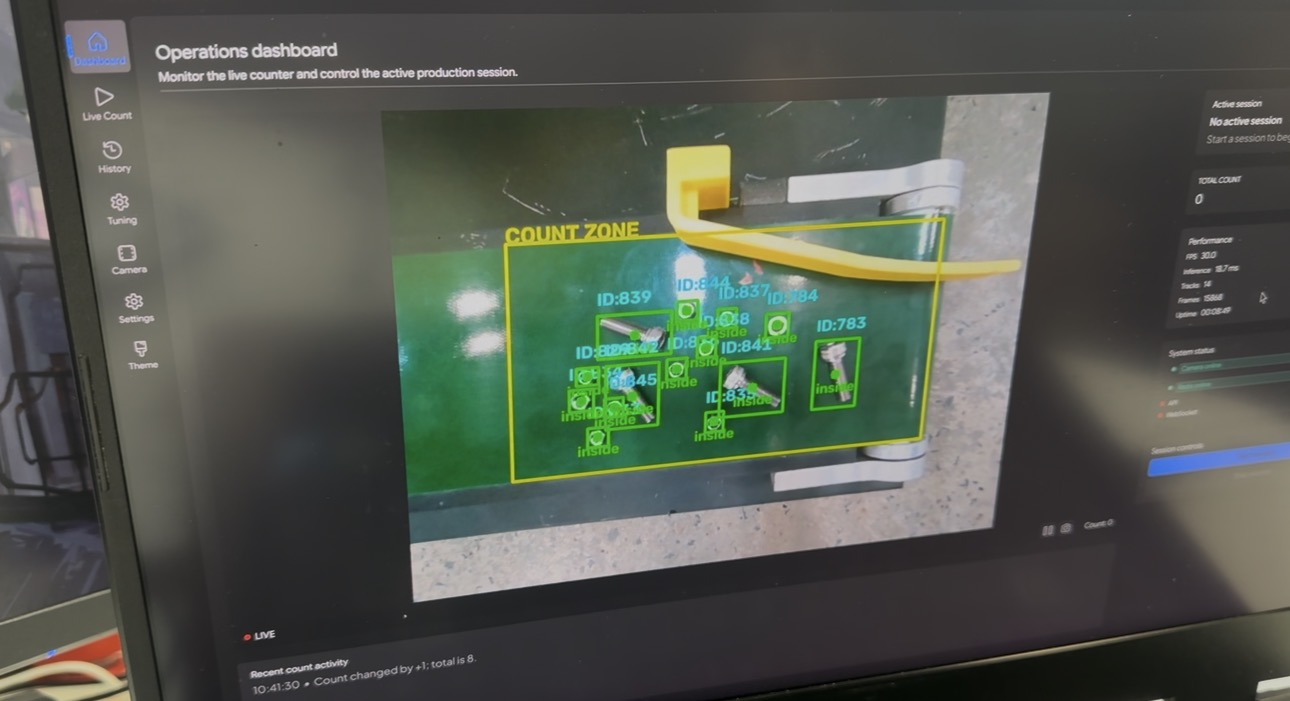
\includegraphics[width=\linewidth]{figures/chapter4/demo.PNG}}
        \caption{System dashboard displaying real-time tally}
    \end{subfigure}
    \hfill
    \begin{subfigure}{0.48\textwidth}
        \centering
        \fbox{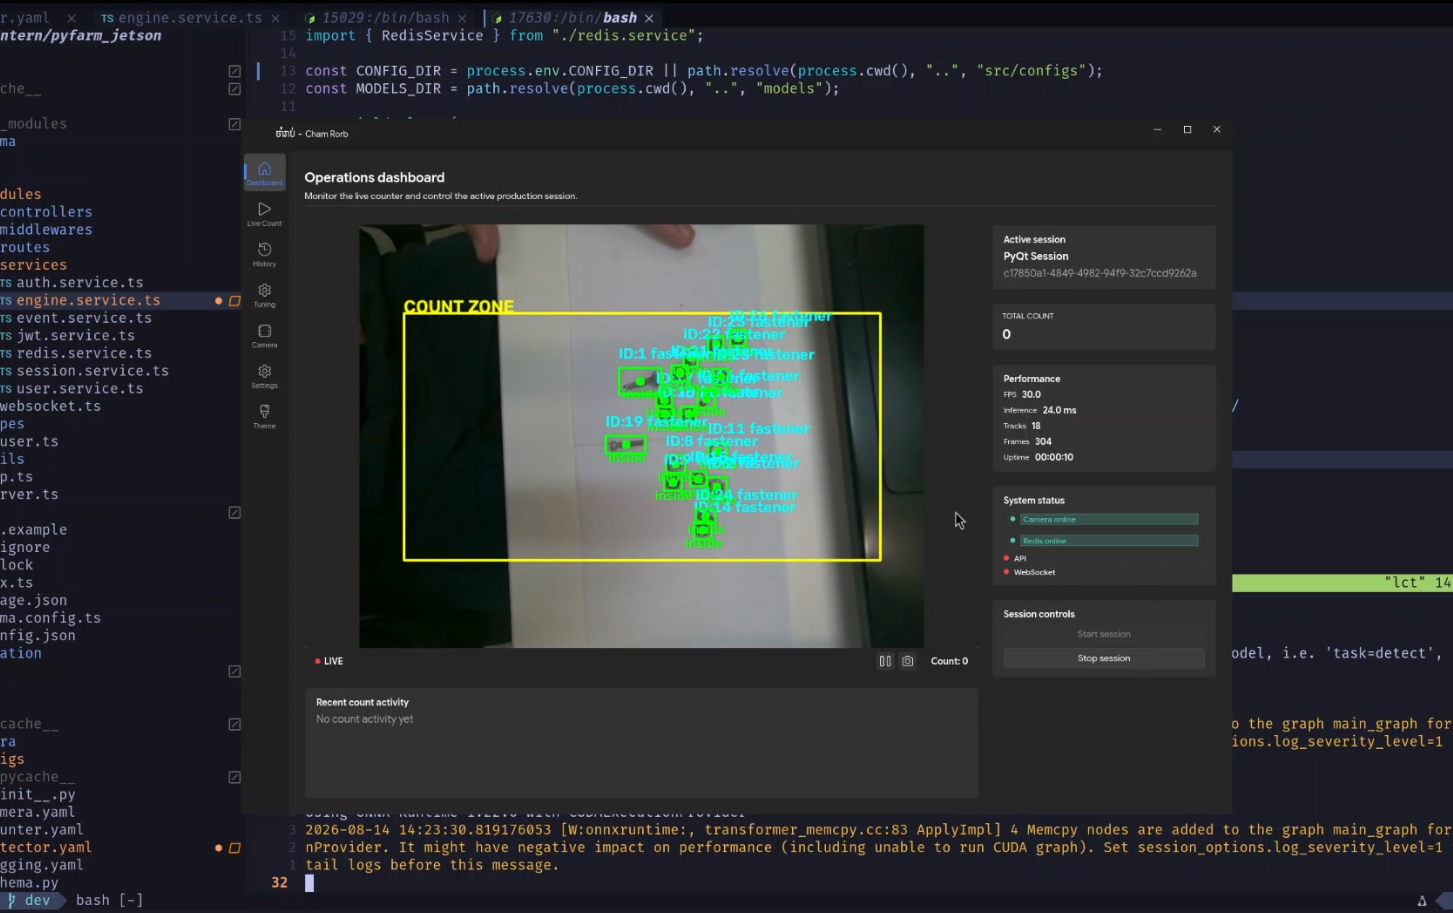
\includegraphics[width=\linewidth]{figures/chapter4/office.png}}
        \caption{High-density fastener with dynamic background}
    \end{subfigure}
    \hfill
    \begin{subfigure}{0.48\textwidth}
        \centering
        \fbox{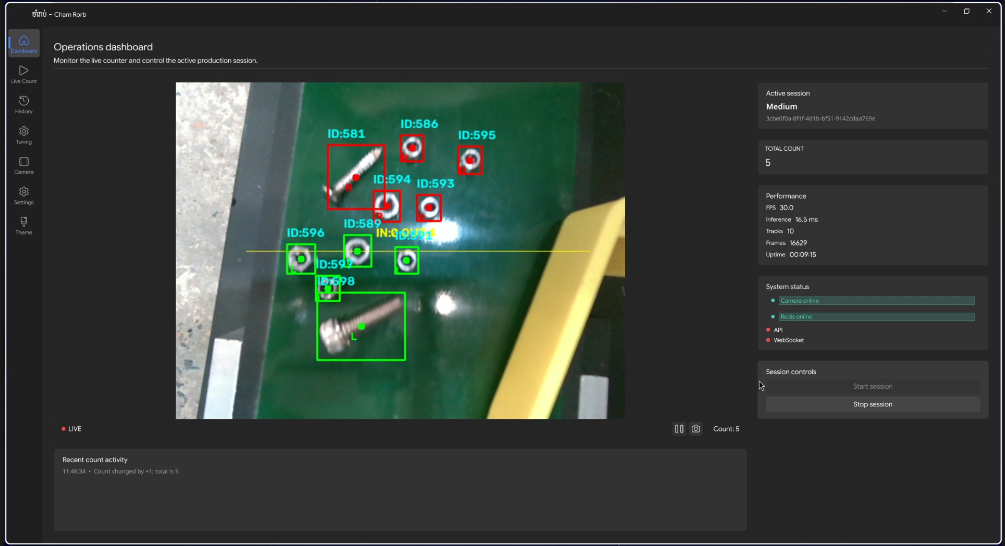
\includegraphics[width=\linewidth]{figures/chapter4/image.png}}
        \caption{Normal fastener flow with occlusion}
    \end{subfigure}
    \caption{Close-up views of the PoC demonstration, highlighting the model's ability to resolve overlapping objects and the corresponding real-time counting interface.}
    \label{fig:poc_details}
\end{figure}

% Optional: If you have a video, you can include it using the media9 or video package
% \begin{figure}[htbp]
%     \centering
%     \includemedia[
%       width=0.8\linewidth,
%       height=0.45\linewidth,
%       activate=pageopen,
%       addresource=figures/chapter4/poc_demo.mp4,
%       flashvars={source=figures/chapter4/poc_demo.mp4}
%     ]{}{VPlayer.swf}
%     \caption{Video recording of the PoC demonstration showing real-time tracking and counting.}
%     \label{fig:poc_video}
% \end{figure}

\section{Edge Deployment Performance Analysis}
The transition from PyTorch training to edge deployment was facilitated by the TensorRT optimization pipeline. Running on the target NVIDIA Jetson platform, the YOLO11-GED model (exported to FP16 precision) achieved the latency and FPS metrics reported in Tables~\ref{tab:benchmark_medium} and \ref{tab:benchmark_hard}.

In the real deployment scenario, the system will be deployed in a close-up configuration where lighting and camera angles are more controlled, which is expected to further improve detection accuracy and reduce false negatives. \\

As observed from the challenging lighting and camera conditions shown in Figure~\ref{fig:poc_details}, the YOLO11-GED (Proposed) model still maintains robust recognition of fastener features and is able to detect and track them. The model's robustness to occlusion, motion blur, and varying object densities confirms the effectiveness of the EMAc2f attention mechanism and DySample upsampling in preserving critical spatial features.\\

Crucially, the system maintained low hardware utilization (GPU Util $\approx$\,37--40\%, CPU Util $\approx$\,8\%), leaving substantial computational headroom for concurrent tasks such as the ByteTrack association algorithm, geometric counting logic, and UI rendering. This confirms that the \texttt{GhostBottleneck} and strategic module placement successfully achieved the design objective of real-time throughput on resource-constrained edge devices.

\section{Summary}
This chapter presented the comprehensive evaluation of the proposed fastener detection and counting system. Quantitative benchmarking on a physical mock-up demonstrated that the proposed YOLO11-GED architecture achieves the optimal balance of speed, efficiency, and accuracy, outperforming both heavier transformer-based baselines and standard YOLO variants in dense scenarios.

Furthermore, the successful Proof of Concept demonstration on a simplified conveyor system validated the model's strong generalization capabilities. Despite being trained on mock-up and public data prior to the completion of the full-scale industrial infrastructure, the system accurately recognized, tracked, and counted fasteners in a near-actual deployment environment. These results confirm that the proposed methodology, architecture, and edge deployment pipeline are robust, practical, and ready for integration into the final industrial conveyor system upon its completion.